\documentclass{article} % For LaTeX2e
% Compile with XeLaTeX (Vietnamese text):  latexmk -xelatex Group06_FinalReport.tex
\usepackage{iclr2027_conference}
\usepackage{fontspec}
\setmainfont{texgyretermes}[Extension=.otf, UprightFont=*-regular, BoldFont=*-bold, ItalicFont=*-italic, BoldItalicFont=*-bolditalic]
%%%%% NEW MATH DEFINITIONS %%%%%

\usepackage{amsmath,amsfonts,bm}

% Mark sections of captions for referring to divisions of figures
\newcommand{\figleft}{{\em (Left)}}
\newcommand{\figcenter}{{\em (Center)}}
\newcommand{\figright}{{\em (Right)}}
\newcommand{\figtop}{{\em (Top)}}
\newcommand{\figbottom}{{\em (Bottom)}}
\newcommand{\captiona}{{\em (a)}}
\newcommand{\captionb}{{\em (b)}}
\newcommand{\captionc}{{\em (c)}}
\newcommand{\captiond}{{\em (d)}}

% Highlight a newly defined term
\newcommand{\newterm}[1]{{\bf #1}}


% Figure reference, lower-case.
\def\figref#1{figure~\ref{#1}}
% Figure reference, capital. For start of sentence
\def\Figref#1{Figure~\ref{#1}}
\def\twofigref#1#2{figures \ref{#1} and \ref{#2}}
\def\quadfigref#1#2#3#4{figures \ref{#1}, \ref{#2}, \ref{#3} and \ref{#4}}
% Section reference, lower-case.
\def\secref#1{section~\ref{#1}}
% Section reference, capital.
\def\Secref#1{Section~\ref{#1}}
% Reference to two sections.
\def\twosecrefs#1#2{sections \ref{#1} and \ref{#2}}
% Reference to three sections.
\def\secrefs#1#2#3{sections \ref{#1}, \ref{#2} and \ref{#3}}
% Reference to an equation, lower-case.
\def\eqref#1{equation~\ref{#1}}
% Reference to an equation, upper case
\def\Eqref#1{Equation~\ref{#1}}
% A raw reference to an equation---avoid using if possible
\def\plaineqref#1{\ref{#1}}
% Reference to a chapter, lower-case.
\def\chapref#1{chapter~\ref{#1}}
% Reference to an equation, upper case.
\def\Chapref#1{Chapter~\ref{#1}}
% Reference to a range of chapters
\def\rangechapref#1#2{chapters\ref{#1}--\ref{#2}}
% Reference to an algorithm, lower-case.
\def\algref#1{algorithm~\ref{#1}}
% Reference to an algorithm, upper case.
\def\Algref#1{Algorithm~\ref{#1}}
\def\twoalgref#1#2{algorithms \ref{#1} and \ref{#2}}
\def\Twoalgref#1#2{Algorithms \ref{#1} and \ref{#2}}
% Reference to a part, lower case
\def\partref#1{part~\ref{#1}}
% Reference to a part, upper case
\def\Partref#1{Part~\ref{#1}}
\def\twopartref#1#2{parts \ref{#1} and \ref{#2}}

\def\ceil#1{\lceil #1 \rceil}
\def\floor#1{\lfloor #1 \rfloor}
\def\1{\bm{1}}
\newcommand{\train}{\mathcal{D}}
\newcommand{\valid}{\mathcal{D_{\mathrm{valid}}}}
\newcommand{\test}{\mathcal{D_{\mathrm{test}}}}

\def\eps{{\epsilon}}


% Random variables
\def\reta{{\textnormal{$\eta$}}}
\def\ra{{\textnormal{a}}}
\def\rb{{\textnormal{b}}}
\def\rc{{\textnormal{c}}}
\def\rd{{\textnormal{d}}}
\def\re{{\textnormal{e}}}
\def\rf{{\textnormal{f}}}
\def\rg{{\textnormal{g}}}
\def\rh{{\textnormal{h}}}
\def\ri{{\textnormal{i}}}
\def\rj{{\textnormal{j}}}
\def\rk{{\textnormal{k}}}
\def\rl{{\textnormal{l}}}
% rm is already a command, just don't name any random variables m
\def\rn{{\textnormal{n}}}
\def\ro{{\textnormal{o}}}
\def\rp{{\textnormal{p}}}
\def\rq{{\textnormal{q}}}
\def\rr{{\textnormal{r}}}
\def\rs{{\textnormal{s}}}
\def\rt{{\textnormal{t}}}
\def\ru{{\textnormal{u}}}
\def\rv{{\textnormal{v}}}
\def\rw{{\textnormal{w}}}
\def\rx{{\textnormal{x}}}
\def\ry{{\textnormal{y}}}
\def\rz{{\textnormal{z}}}

% Random vectors
\def\rvepsilon{{\mathbf{\epsilon}}}
\def\rvtheta{{\mathbf{\theta}}}
\def\rva{{\mathbf{a}}}
\def\rvb{{\mathbf{b}}}
\def\rvc{{\mathbf{c}}}
\def\rvd{{\mathbf{d}}}
\def\rve{{\mathbf{e}}}
\def\rvf{{\mathbf{f}}}
\def\rvg{{\mathbf{g}}}
\def\rvh{{\mathbf{h}}}
\def\rvu{{\mathbf{i}}}
\def\rvj{{\mathbf{j}}}
\def\rvk{{\mathbf{k}}}
\def\rvl{{\mathbf{l}}}
\def\rvm{{\mathbf{m}}}
\def\rvn{{\mathbf{n}}}
\def\rvo{{\mathbf{o}}}
\def\rvp{{\mathbf{p}}}
\def\rvq{{\mathbf{q}}}
\def\rvr{{\mathbf{r}}}
\def\rvs{{\mathbf{s}}}
\def\rvt{{\mathbf{t}}}
\def\rvu{{\mathbf{u}}}
\def\rvv{{\mathbf{v}}}
\def\rvw{{\mathbf{w}}}
\def\rvx{{\mathbf{x}}}
\def\rvy{{\mathbf{y}}}
\def\rvz{{\mathbf{z}}}

% Elements of random vectors
\def\erva{{\textnormal{a}}}
\def\ervb{{\textnormal{b}}}
\def\ervc{{\textnormal{c}}}
\def\ervd{{\textnormal{d}}}
\def\erve{{\textnormal{e}}}
\def\ervf{{\textnormal{f}}}
\def\ervg{{\textnormal{g}}}
\def\ervh{{\textnormal{h}}}
\def\ervi{{\textnormal{i}}}
\def\ervj{{\textnormal{j}}}
\def\ervk{{\textnormal{k}}}
\def\ervl{{\textnormal{l}}}
\def\ervm{{\textnormal{m}}}
\def\ervn{{\textnormal{n}}}
\def\ervo{{\textnormal{o}}}
\def\ervp{{\textnormal{p}}}
\def\ervq{{\textnormal{q}}}
\def\ervr{{\textnormal{r}}}
\def\ervs{{\textnormal{s}}}
\def\ervt{{\textnormal{t}}}
\def\ervu{{\textnormal{u}}}
\def\ervv{{\textnormal{v}}}
\def\ervw{{\textnormal{w}}}
\def\ervx{{\textnormal{x}}}
\def\ervy{{\textnormal{y}}}
\def\ervz{{\textnormal{z}}}

% Random matrices
\def\rmA{{\mathbf{A}}}
\def\rmB{{\mathbf{B}}}
\def\rmC{{\mathbf{C}}}
\def\rmD{{\mathbf{D}}}
\def\rmE{{\mathbf{E}}}
\def\rmF{{\mathbf{F}}}
\def\rmG{{\mathbf{G}}}
\def\rmH{{\mathbf{H}}}
\def\rmI{{\mathbf{I}}}
\def\rmJ{{\mathbf{J}}}
\def\rmK{{\mathbf{K}}}
\def\rmL{{\mathbf{L}}}
\def\rmM{{\mathbf{M}}}
\def\rmN{{\mathbf{N}}}
\def\rmO{{\mathbf{O}}}
\def\rmP{{\mathbf{P}}}
\def\rmQ{{\mathbf{Q}}}
\def\rmR{{\mathbf{R}}}
\def\rmS{{\mathbf{S}}}
\def\rmT{{\mathbf{T}}}
\def\rmU{{\mathbf{U}}}
\def\rmV{{\mathbf{V}}}
\def\rmW{{\mathbf{W}}}
\def\rmX{{\mathbf{X}}}
\def\rmY{{\mathbf{Y}}}
\def\rmZ{{\mathbf{Z}}}

% Elements of random matrices
\def\ermA{{\textnormal{A}}}
\def\ermB{{\textnormal{B}}}
\def\ermC{{\textnormal{C}}}
\def\ermD{{\textnormal{D}}}
\def\ermE{{\textnormal{E}}}
\def\ermF{{\textnormal{F}}}
\def\ermG{{\textnormal{G}}}
\def\ermH{{\textnormal{H}}}
\def\ermI{{\textnormal{I}}}
\def\ermJ{{\textnormal{J}}}
\def\ermK{{\textnormal{K}}}
\def\ermL{{\textnormal{L}}}
\def\ermM{{\textnormal{M}}}
\def\ermN{{\textnormal{N}}}
\def\ermO{{\textnormal{O}}}
\def\ermP{{\textnormal{P}}}
\def\ermQ{{\textnormal{Q}}}
\def\ermR{{\textnormal{R}}}
\def\ermS{{\textnormal{S}}}
\def\ermT{{\textnormal{T}}}
\def\ermU{{\textnormal{U}}}
\def\ermV{{\textnormal{V}}}
\def\ermW{{\textnormal{W}}}
\def\ermX{{\textnormal{X}}}
\def\ermY{{\textnormal{Y}}}
\def\ermZ{{\textnormal{Z}}}

% Vectors
\def\vzero{{\bm{0}}}
\def\vone{{\bm{1}}}
\def\vmu{{\bm{\mu}}}
\def\vtheta{{\bm{\theta}}}
\def\va{{\bm{a}}}
\def\vb{{\bm{b}}}
\def\vc{{\bm{c}}}
\def\vd{{\bm{d}}}
\def\ve{{\bm{e}}}
\def\vf{{\bm{f}}}
\def\vg{{\bm{g}}}
\def\vh{{\bm{h}}}
\def\vi{{\bm{i}}}
\def\vj{{\bm{j}}}
\def\vk{{\bm{k}}}
\def\vl{{\bm{l}}}
\def\vm{{\bm{m}}}
\def\vn{{\bm{n}}}
\def\vo{{\bm{o}}}
\def\vp{{\bm{p}}}
\def\vq{{\bm{q}}}
\def\vr{{\bm{r}}}
\def\vs{{\bm{s}}}
\def\vt{{\bm{t}}}
\def\vu{{\bm{u}}}
\def\vv{{\bm{v}}}
\def\vw{{\bm{w}}}
\def\vx{{\bm{x}}}
\def\vy{{\bm{y}}}
\def\vz{{\bm{z}}}

% Elements of vectors
\def\evalpha{{\alpha}}
\def\evbeta{{\beta}}
\def\evepsilon{{\epsilon}}
\def\evlambda{{\lambda}}
\def\evomega{{\omega}}
\def\evmu{{\mu}}
\def\evpsi{{\psi}}
\def\evsigma{{\sigma}}
\def\evtheta{{\theta}}
\def\eva{{a}}
\def\evb{{b}}
\def\evc{{c}}
\def\evd{{d}}
\def\eve{{e}}
\def\evf{{f}}
\def\evg{{g}}
\def\evh{{h}}
\def\evi{{i}}
\def\evj{{j}}
\def\evk{{k}}
\def\evl{{l}}
\def\evm{{m}}
\def\evn{{n}}
\def\evo{{o}}
\def\evp{{p}}
\def\evq{{q}}
\def\evr{{r}}
\def\evs{{s}}
\def\evt{{t}}
\def\evu{{u}}
\def\evv{{v}}
\def\evw{{w}}
\def\evx{{x}}
\def\evy{{y}}
\def\evz{{z}}

% Matrix
\def\mA{{\bm{A}}}
\def\mB{{\bm{B}}}
\def\mC{{\bm{C}}}
\def\mD{{\bm{D}}}
\def\mE{{\bm{E}}}
\def\mF{{\bm{F}}}
\def\mG{{\bm{G}}}
\def\mH{{\bm{H}}}
\def\mI{{\bm{I}}}
\def\mJ{{\bm{J}}}
\def\mK{{\bm{K}}}
\def\mL{{\bm{L}}}
\def\mM{{\bm{M}}}
\def\mN{{\bm{N}}}
\def\mO{{\bm{O}}}
\def\mP{{\bm{P}}}
\def\mQ{{\bm{Q}}}
\def\mR{{\bm{R}}}
\def\mS{{\bm{S}}}
\def\mT{{\bm{T}}}
\def\mU{{\bm{U}}}
\def\mV{{\bm{V}}}
\def\mW{{\bm{W}}}
\def\mX{{\bm{X}}}
\def\mY{{\bm{Y}}}
\def\mZ{{\bm{Z}}}
\def\mBeta{{\bm{\beta}}}
\def\mPhi{{\bm{\Phi}}}
\def\mLambda{{\bm{\Lambda}}}
\def\mSigma{{\bm{\Sigma}}}

% Tensor
\DeclareMathAlphabet{\mathsfit}{\encodingdefault}{\sfdefault}{m}{sl}
\SetMathAlphabet{\mathsfit}{bold}{\encodingdefault}{\sfdefault}{bx}{n}
\newcommand{\tens}[1]{\bm{\mathsfit{#1}}}
\def\tA{{\tens{A}}}
\def\tB{{\tens{B}}}
\def\tC{{\tens{C}}}
\def\tD{{\tens{D}}}
\def\tE{{\tens{E}}}
\def\tF{{\tens{F}}}
\def\tG{{\tens{G}}}
\def\tH{{\tens{H}}}
\def\tI{{\tens{I}}}
\def\tJ{{\tens{J}}}
\def\tK{{\tens{K}}}
\def\tL{{\tens{L}}}
\def\tM{{\tens{M}}}
\def\tN{{\tens{N}}}
\def\tO{{\tens{O}}}
\def\tP{{\tens{P}}}
\def\tQ{{\tens{Q}}}
\def\tR{{\tens{R}}}
\def\tS{{\tens{S}}}
\def\tT{{\tens{T}}}
\def\tU{{\tens{U}}}
\def\tV{{\tens{V}}}
\def\tW{{\tens{W}}}
\def\tX{{\tens{X}}}
\def\tY{{\tens{Y}}}
\def\tZ{{\tens{Z}}}


% Graph
\def\gA{{\mathcal{A}}}
\def\gB{{\mathcal{B}}}
\def\gC{{\mathcal{C}}}
\def\gD{{\mathcal{D}}}
\def\gE{{\mathcal{E}}}
\def\gF{{\mathcal{F}}}
\def\gG{{\mathcal{G}}}
\def\gH{{\mathcal{H}}}
\def\gI{{\mathcal{I}}}
\def\gJ{{\mathcal{J}}}
\def\gK{{\mathcal{K}}}
\def\gL{{\mathcal{L}}}
\def\gM{{\mathcal{M}}}
\def\gN{{\mathcal{N}}}
\def\gO{{\mathcal{O}}}
\def\gP{{\mathcal{P}}}
\def\gQ{{\mathcal{Q}}}
\def\gR{{\mathcal{R}}}
\def\gS{{\mathcal{S}}}
\def\gT{{\mathcal{T}}}
\def\gU{{\mathcal{U}}}
\def\gV{{\mathcal{V}}}
\def\gW{{\mathcal{W}}}
\def\gX{{\mathcal{X}}}
\def\gY{{\mathcal{Y}}}
\def\gZ{{\mathcal{Z}}}

% Sets
\def\sA{{\mathbb{A}}}
\def\sB{{\mathbb{B}}}
\def\sC{{\mathbb{C}}}
\def\sD{{\mathbb{D}}}
% Don't use a set called E, because this would be the same as our symbol
% for expectation.
\def\sF{{\mathbb{F}}}
\def\sG{{\mathbb{G}}}
\def\sH{{\mathbb{H}}}
\def\sI{{\mathbb{I}}}
\def\sJ{{\mathbb{J}}}
\def\sK{{\mathbb{K}}}
\def\sL{{\mathbb{L}}}
\def\sM{{\mathbb{M}}}
\def\sN{{\mathbb{N}}}
\def\sO{{\mathbb{O}}}
\def\sP{{\mathbb{P}}}
\def\sQ{{\mathbb{Q}}}
\def\sR{{\mathbb{R}}}
\def\sS{{\mathbb{S}}}
\def\sT{{\mathbb{T}}}
\def\sU{{\mathbb{U}}}
\def\sV{{\mathbb{V}}}
\def\sW{{\mathbb{W}}}
\def\sX{{\mathbb{X}}}
\def\sY{{\mathbb{Y}}}
\def\sZ{{\mathbb{Z}}}

% Entries of a matrix
\def\emLambda{{\Lambda}}
\def\emA{{A}}
\def\emB{{B}}
\def\emC{{C}}
\def\emD{{D}}
\def\emE{{E}}
\def\emF{{F}}
\def\emG{{G}}
\def\emH{{H}}
\def\emI{{I}}
\def\emJ{{J}}
\def\emK{{K}}
\def\emL{{L}}
\def\emM{{M}}
\def\emN{{N}}
\def\emO{{O}}
\def\emP{{P}}
\def\emQ{{Q}}
\def\emR{{R}}
\def\emS{{S}}
\def\emT{{T}}
\def\emU{{U}}
\def\emV{{V}}
\def\emW{{W}}
\def\emX{{X}}
\def\emY{{Y}}
\def\emZ{{Z}}
\def\emSigma{{\Sigma}}

% entries of a tensor
% Same font as tensor, without \bm wrapper
\newcommand{\etens}[1]{\mathsfit{#1}}
\def\etLambda{{\etens{\Lambda}}}
\def\etA{{\etens{A}}}
\def\etB{{\etens{B}}}
\def\etC{{\etens{C}}}
\def\etD{{\etens{D}}}
\def\etE{{\etens{E}}}
\def\etF{{\etens{F}}}
\def\etG{{\etens{G}}}
\def\etH{{\etens{H}}}
\def\etI{{\etens{I}}}
\def\etJ{{\etens{J}}}
\def\etK{{\etens{K}}}
\def\etL{{\etens{L}}}
\def\etM{{\etens{M}}}
\def\etN{{\etens{N}}}
\def\etO{{\etens{O}}}
\def\etP{{\etens{P}}}
\def\etQ{{\etens{Q}}}
\def\etR{{\etens{R}}}
\def\etS{{\etens{S}}}
\def\etT{{\etens{T}}}
\def\etU{{\etens{U}}}
\def\etV{{\etens{V}}}
\def\etW{{\etens{W}}}
\def\etX{{\etens{X}}}
\def\etY{{\etens{Y}}}
\def\etZ{{\etens{Z}}}

% The true underlying data generating distribution
\newcommand{\pdata}{p_{\rm{data}}}
% The empirical distribution defined by the training set
\newcommand{\ptrain}{\hat{p}_{\rm{data}}}
\newcommand{\Ptrain}{\hat{P}_{\rm{data}}}
% The model distribution
\newcommand{\pmodel}{p_{\rm{model}}}
\newcommand{\Pmodel}{P_{\rm{model}}}
\newcommand{\ptildemodel}{\tilde{p}_{\rm{model}}}
% Stochastic autoencoder distributions
\newcommand{\pencode}{p_{\rm{encoder}}}
\newcommand{\pdecode}{p_{\rm{decoder}}}
\newcommand{\precons}{p_{\rm{reconstruct}}}

\newcommand{\laplace}{\mathrm{Laplace}} % Laplace distribution

\newcommand{\E}{\mathbb{E}}
\newcommand{\Ls}{\mathcal{L}}
\newcommand{\R}{\mathbb{R}}
\newcommand{\emp}{\tilde{p}}
\newcommand{\lr}{\alpha}
\newcommand{\reg}{\lambda}
\newcommand{\rect}{\mathrm{rectifier}}
\newcommand{\softmax}{\mathrm{softmax}}
\newcommand{\sigmoid}{\sigma}
\newcommand{\softplus}{\zeta}
\newcommand{\KL}{D_{\mathrm{KL}}}
\newcommand{\Var}{\mathrm{Var}}
\newcommand{\standarderror}{\mathrm{SE}}
\newcommand{\Cov}{\mathrm{Cov}}
% Wolfram Mathworld says $L^2$ is for function spaces and $\ell^2$ is for vectors
% But then they seem to use $L^2$ for vectors throughout the site, and so does
% wikipedia.
\newcommand{\normlzero}{L^0}
\newcommand{\normlone}{L^1}
\newcommand{\normltwo}{L^2}
\newcommand{\normlp}{L^p}
\newcommand{\normmax}{L^\infty}

\newcommand{\parents}{Pa} % See usage in notation.tex. Chosen to match Daphne's book.

\DeclareMathOperator*{\argmax}{arg\,max}
\DeclareMathOperator*{\argmin}{arg\,min}

\DeclareMathOperator{\sign}{sign}
\DeclareMathOperator{\Tr}{Tr}
\let\ab\allowbreak


\usepackage{hyperref}
\usepackage{url}
\usepackage{booktabs}
\usepackage{multirow}
\usepackage{graphicx}
\usepackage{xcolor}
\usepackage{enumitem}
\usepackage{float}
\usepackage{wrapfig}
\usepackage{amsmath}
\setlist{nosep, leftmargin=1.2em}
\setlength{\textfloatsep}{8pt plus 2pt minus 2pt}
\setlength{\floatsep}{16pt plus 3pt minus 2pt}
\setlength{\intextsep}{7pt plus 2pt minus 2pt}
\setlength{\abovecaptionskip}{3pt}
\setlength{\belowcaptionskip}{2pt}
\usepackage{tikz}
\usetikzlibrary{arrows.meta,positioning,calc,shapes.misc}
\usepackage{pgfplots}
\pgfplotsset{compat=1.18}
\definecolor{cblue}{HTML}{1F5F8B}
\definecolor{cred}{HTML}{9B2C2C}
\definecolor{cgreen}{HTML}{2F7D4F}
\definecolor{camber}{HTML}{B7791F}
\definecolor{cgray}{HTML}{A0A7B2}
\definecolor{cpurple}{HTML}{6B4C9A}
\pgfplotsset{lexstyle/.style={
  font=\scriptsize, tick label style={font=\scriptsize}, label style={font=\scriptsize},
  legend style={font=\scriptsize, draw=none, fill=none},
  axis line style={black!60}, tick style={black!60}, major grid style={black!12}, tick pos=left}}
\newcommand{\cur}{_{\text{cur}}}

% generated by scripts/make_report_results.py -- do not edit by hand
\newcommand{\ResZsMrr}{0.539}
\newcommand{\ResZsRten}{0.742}
\newcommand{\ResZsCeMrr}{0.624}
\newcommand{\ResZsCeRten}{0.792}
\newcommand{\ResFtMrr}{0.650}
\newcommand{\ResFtRten}{0.865}
\newcommand{\ResFtCeMrr}{0.704}
\newcommand{\ResFtCeRten}{0.885}
\newcommand{\ResStaleNoTime}{0.234}
\newcommand{\ResStaleTime}{0.125}
\newcommand{\ResTmrrNoTime}{0.377}
\newcommand{\ResTmrrTime}{0.486}
\newcommand{\ResThitNoTime}{0.692}
\newcommand{\ResThitTime}{0.744}
\newcommand{\ResNTemporal}{1,913}
\newcommand{\ResStaleNoTimePct}{23\%}
\newcommand{\ResStaleTimePct}{12.5\%}
\newcommand{\ResTimeMrr}{0.671}
\newcommand{\ResTmrrAmends}{0.468}
\newcommand{\ResTmrrRepl}{0.472}
\newcommand{\ResWeights}{$\gamma=2$}
\newcommand{\ResCePairs}{445,296}
\newcommand{\ResAblRows}{fine-tuned retriever + re-ranker (no time signals) & 0.704 & 0.667 & 0.234 & 0.377 & 0.692 \\
\quad \textbf{+ time signals (stale penalty, successor injection)} & 0.671 & 0.681 & 0.125 & 0.486 & 0.744 \\
\midrule
\quad + stale penalty only (no successor injection) & 0.671 & 0.681 & 0.127 & 0.481 & 0.721 \\
\quad + time signals, amends edges only & 0.676 & 0.677 & 0.117 & 0.468 & 0.725 \\
\quad + time signals, replaces / repeals edges only & 0.675 & 0.678 & 0.119 & 0.472 & 0.736 \\}
\newcommand{\ResLlmRows}{no retrieval & -- & 0.120 & 0.000 & 0.600 \\
plain RAG & 0.420 & 0.640 & 0.000 & 0.950 \\
time-aware RAG (ours) & 0.513 & 0.693 & 0.640 & 0.950 \\}
\newcommand{\ResNAns}{170}
\newcommand{\ResLlmFullRows}{no retrieval & -- & 0.120 & 0.080 & 0.020 & 0.000 & 0.000 & 0.600 \\
plain RAG & 0.420 & 0.640 & 0.580 & 0.693 & 0.000 & 0.000 & 0.950 \\
\textbf{time-aware RAG (ours)} & 0.513 & 0.693 & 0.660 & 0.707 & 0.731 & 0.130 & 0.950 \\}
\newcommand{\ResNChanged}{26}
\newcommand{\ResAlignAcc}{0.730}
\newcommand{\ResAlignAccPct}{73\%}
\newcommand{\ResAnsFalseAlarm}{0.130}
\newcommand{\ResAnsFalseAlarmPct}{13\%}
\newcommand{\ResAnsNoticeRecall}{0.731}
\newcommand{\ResAnsNoticeRecallPct}{73\%}
\newcommand{\ResAnsCorrect}{0.693}
\newcommand{\ResAnsCorrectPct}{69\%}
\newcommand{\ResAnsCorrectT}{0.660}
\newcommand{\ResAnsCorrectTPct}{66\%}
\newcommand{\ResAnsNoticeT}{0.640}
\newcommand{\ResAnsNoticeTPct}{64\%}
\newcommand{\ResAnsPlainCorrect}{0.640}
\newcommand{\ResAnsPlainCorrectT}{0.580}
\newcommand{\ResAnsNoneCorrectPct}{12\%}
\newcommand{\ResTtRows}{static RAG & 0.917 & 0.060 & 0.059 \\
no time signals & 0.849 & 0.620 & 0.583 \\
LexGraph-VN & 0.873 & 0.679 & 0.651 \\}
\newcommand{\ResNTt}{1,752}
\newcommand{\ResTtBothPct}{65\%}
\newcommand{\ResTtStaticBothPct}{6\%}
\newcommand{\ResBiCurve}{(0.000,0.6193) (0.242,0.7131) (0.484,0.7277) (0.726,0.7393) (0.967,0.7405) (1.000,0.7409)}
\newcommand{\ResCeCurve}{(0.000,0.7285) (0.144,0.7886) (0.288,0.7868) (0.431,0.7866) (0.575,0.8014) (0.719,0.8081) (0.863,0.8063) (1.000,0.8057)}
\newcommand{\ResMuCurve}{(0,0.6991)}
\newcommand{\ResGammaMrr}{(0,0.6879) (0.5,0.6951) (1,0.6980) (2,0.6991) (4,0.6862) (8,0.6538)}
\newcommand{\ResGammaStale}{(0,0.2283) (0.5,0.1955) (1,0.1683) (2,0.1241) (4,0.0653) (8,0.0185)}
\newcommand{\ResAlignHistRej}{(0.025,41586) (0.075,4557) (0.125,2739) (0.175,2030) (0.225,1677) (0.275,1429) (0.325,1286) (0.375,1161) (0.425,1089) (0.475,1019) (0.525,1049) (0.575,987) (0.625,1001) (0.675,966) (0.725,1001) (0.775,1092) (0.825,624) (0.875,708) (0.925,798) (0.975,1533)}
\newcommand{\ResAlignHistAcc}{(0.025,0) (0.075,0) (0.125,0) (0.175,0) (0.225,0) (0.275,0) (0.325,0) (0.375,0) (0.425,0) (0.475,0) (0.525,0) (0.575,0) (0.625,0) (0.675,0) (0.725,0) (0.775,0) (0.825,496) (0.875,640) (0.925,1010) (0.975,5319)}
\newcommand{\ResAlignThr}{0.80}
\newcommand{\ResAlignAccepted}{9,362}
\newcommand{\ResAlignPairs}{31,574}
\newcommand{\ResAlignArtPairs}{75,797}
\newcommand{\ResAlignArtAccepted}{7,465}
\newcommand{\ResAlignJudged}{2,359}
\newcommand{\ResAlignPrec}{0.88}
\newcommand{\ResAlignRec}{0.33}
\newcommand{\ResTtSt}{(before,0.917) (after,0.060) (both,0.059)}
\newcommand{\ResTtNt}{(before,0.849) (after,0.620) (both,0.583)}
\newcommand{\ResTtLg}{(before,0.873) (after,0.679) (both,0.651)}
\newcommand{\ResAnsNone}{(correct,0.120) (temporal,0.080) (notice,0.000) (refuse,0.600)}
\newcommand{\ResAnsPlain}{(correct,0.640) (temporal,0.580) (notice,0.000) (refuse,0.950)}
\newcommand{\ResAnsOurs}{(correct,0.693) (temporal,0.660) (notice,0.640) (refuse,0.950)}
\newcommand{\ResFindings}{(to be written from the final numbers)}

% generated by scripts/make_final_report_data.py -- do not edit by hand
\newcommand{\KgEdgeSyms}{basedon,cites,repeals,guides,replaces,amends,partiallyrepeals,suspends,interprets}
\newcommand{\KgEdgeLabels}{{based on},{cites},{repeals},{guides},{replaces},{amends},{part.\ repeals},{suspends},{interprets}}
\newcommand{\KgEdgeCoords}{(663907,basedon) (65586,cites) (61872,repeals) (41641,guides) (36829,replaces) (17665,amends) (6557,partiallyrepeals) (188,suspends) (85,interprets)}
\newcommand{\KgInForcePct}{40.4}
\newcommand{\KgExpiredPct}{55.4}
\newcommand{\KgPartlyPct}{3.5}
\newcommand{\KgTypeDecision}{91,183}
\newcommand{\KgTypeResolution}{28,337}
\newcommand{\KgTypeCircular}{17,232}
\newcommand{\KgTypeDecree}{5,328}
\newcommand{\KgTypeLaw}{610}
\newcommand{\KgTypeJointCircular}{3,519}
\newcommand{\KgTypeOrdinance}{248}
\newcommand{\KgLouvainComm}{151}
\newcommand{\KgLouvainMod}{0.58}
\newcommand{\KgLouvainNodes}{82,945}
\newcommand{\KgXrefP}{0.63}
\newcommand{\KgXrefR}{0.51}
\newcommand{\KgXrefNew}{215,573}
\newcommand{\KgArtXref}{105,307}
\newcommand{\KgArtXrefRes}{89.4}
\newcommand{\KgDocsWithArticles}{127,802}
\newcommand{\KgAuthRows}{1 & 77/2015/QH13 & Tổ chức chính quyền địa phương \\
2 & 80/2015/QH13 & Ban hành văn bản quy phạm pháp luật \\
3 & 47/2019/QH14 & Luật sửa đổi, bổ sung một số điều của Luật Tổ chức Chính p… \\
4 & 63/2020/QH14 & sửa đổi, bổ sung một số điều của Luật Ban hành văn bản quy… \\
5 & 83/2015/QH13 & Ngân sách nhà nước \\
6 & 34/2016/NĐ-CP & Quy định chi tiết một số điều và biện pháp thi hành L \\}
\newcommand{\KgCommRows}{17,685 & Ngân sách nhà nước; Tổ chức- Biên chế \\
13,223 & Lao động, tiền lương, tiền công; Đất đai \\
12,078 & Quản lý thuế, phí và lệ phí; Quản lý thuế, phí, lệ phí và thu khác của ngân sách nhà nước \\
4,976 & Xuất nhập khẩu; Tiêu chuẩn đo lường chất lượng \\
4,176 & Đất đai; Lĩnh vực giá \\
3,734 & Xây dựng; Quản lý hoạt động xây dựng \\}
\newcommand{\EdaQWords}{20.3}
\newcommand{\EdaPWords}{220}
\newcommand{\EdaPWordsNinetyNine}{844}
\newcommand{\EdaUnseen}{40\%}
\newcommand{\EdaMultiGold}{10.1\%}
\newcommand{\BaseRows}{BM25 (syllables) & 0.471 & 0.671 & 0.851 \\
BM25 (pyvi words) & 0.491 & 0.702 & 0.880 \\
vietnamese-bi-encoder & 0.557 & 0.759 & 0.903 \\
BGE-M3 (zero-shot) & 0.608 & 0.804 & 0.939 \\
BGE-M3 (fine-tuned) & 0.725 & 0.909 & 0.985 \\}
\newcommand{\AlFeatSyms}{sim,tokjacc,ce,rank,headjacc,lenratio,artdist,relrepeals}
\newcommand{\AlFeatLabels}{{bi-encoder similarity},{token overlap},{cross-encoder score},{candidate rank},{heading overlap},{length ratio},{article-number distance},{relation: repeals}}
\newcommand{\AlFeatCoords}{(0.1118,sim) (0.0452,tokjacc) (0.0377,ce) (0.0263,rank) (0.0211,headjacc) (0.0211,lenratio) (0.0154,artdist) (0.0057,relrepeals)}
\newcommand{\AlTestAcc}{0.79}
\newcommand{\AlTestF}{0.48}
\newcommand{\AlClsP}{0.83}
\newcommand{\AlClsR}{0.49}
\newcommand{\AlPosRate}{31\%}
\newcommand{\AlSplits}{1,477 / 426 / 456}
\newcommand{\NoticeNone}{(11.7,70.1) (13.0,80.5) (14.0,86.2) (14.0,88.5) (14.7,89.7) (15.0,89.7) (15.3,89.7)}
\newcommand{\NoticeFast}{(9.7,63.2) (10.7,73.6) (11.7,79.3) (11.7,82.8) (12.0,83.9) (12.3,83.9) (12.3,83.9)}
\newcommand{\NoticeThink}{(7.3,46.0) (8.0,52.9) (8.3,56.3) (8.3,59.8) (8.3,60.9) (8.3,60.9) (8.3,60.9)}
\newcommand{\NoticeNChanged}{87}
\newcommand{\ParserRows}{document number & 98.8 & 242 \\
title & 99.6 & 242 \\
document type & 100.0 & 242 \\
issuing body & 91.3 & 242 \\
issue date & 100.0 & 241 \\
effective date & 100.0 & 231 \\
expiry date & 97.8 & 91 \\
validity status & 93.0 & 242 \\
number of articles & 91.0 & 166 \\}
\newcommand{\ParserSyms}{p0,p1,p2,p3,p4,p5,p6,p7,p8}
\newcommand{\ParserLabels}{{number},{title},{type},{issue date},{effective date},{expiry date},{status},{issuing body},{no.\ of articles}}
\newcommand{\ParserCoords}{(98.8,p0) (99.6,p1) (100.0,p2) (100.0,p3) (100.0,p4) (97.8,p5) (93.0,p6) (91.3,p7) (91.0,p8)}
\newcommand{\ParserDocs}{242}
\newcommand{\RelRows}{any type & 0.76 & 0.83 & 808 \\
based on & 0.88 & 0.78 & 607 \\
succession & 0.58 & 0.55 & 123 \\
replaces / repeals & 0.53 & 0.46 & 91 \\}
\newcommand{\RelSyms}{r0,r1,r2,r3}
\newcommand{\RelLabels}{{any type},{based on},{succession},{replaces/repeals}}
\newcommand{\RelP}{(r0,0.76) (r1,0.88) (r2,0.58) (r3,0.53)}
\newcommand{\RelR}{(r0,0.83) (r1,0.78) (r2,0.55) (r3,0.46)}
\newcommand{\CrawlFetched}{1,087}
\newcommand{\CrawlParsed}{978}
\newcommand{\CrawlBlocked}{0}
\newcommand{\LiveNewDocs}{645}
\newcommand{\LiveNewArts}{11,795}
\newcommand{\LiveNewEdges}{6,178}
\newcommand{\LiveNewOps}{1,057}
\newcommand{\LiveClosed}{367}
\newcommand{\LiveNewChunks}{21,000}
\newcommand{\LiveNewAlign}{1,270}
\newcommand{\LiveAffected}{3,581}
\newcommand{\AmOps}{38,344}
\newcommand{\AmDocs}{6,117}
\newcommand{\AmResolved}{92.0}
\newcommand{\AmArtFound}{67.7}
\newcommand{\AmOpCoords}{(17053,{Sửa đổi, bổ sung}) (8112,{Sửa đổi}) (6066,{Bổ sung}) (3398,{Bãi bỏ}) (2706,{Thay thế}) (942,{Thay cụm từ})}
\newcommand{\FmSyms}{f0,f1,f2,f3,f4,f5}
\newcommand{\FmLabels}{{wrong clause / number},{incomplete rule},{unsupported claim},{retrieval miss},{outdated source cited},{wrong refusal}}
\newcommand{\FmCoords}{(14,f0) (11,f1) (8,f2) (7,f3) (3,f4) (3,f5)}
\newcommand{\FmWrong}{46}
\newcommand{\FmInScope}{150}
\newcommand{\FmMisread}{33}
\newcommand{\FmRetrieval}{7}
\newcommand{\FmOutdated}{3}
\newcommand{\FmRefusal}{3}
\newcommand{\FmClause}{14}
\newcommand{\FmIncomplete}{11}
\newcommand{\FmUnsupported}{8}
\newcommand{\FmFalse}{13}
\newcommand{\FmMissed}{7}
\newcommand{\FmMissedNoFact}{7}
\newcommand{\FmChanged}{26}
\newcommand{\JTwoRows}{no retrieval & -- & 0.173 & 0.120 & 0.040 & 0.000 & 0.000 & -- \\
plain RAG & -- & 0.647 & 0.540 & 0.680 & 0.000 & 0.000 & -- \\
\textbf{time-aware RAG (ours)} & -- & 0.773 & 0.800 & 0.767 & 0.714 & 0.130 & -- \\}
\newcommand{\JTwoKappaCorrect}{0.58}
\newcommand{\JTwoAgreeCorrect}{79\%}
\newcommand{\JTwoKappaFaithful}{0.65}
\newcommand{\JTwoAgreeFaithful}{83\%}
\newcommand{\JTwoKappaChanged}{0.60}
\newcommand{\JTwoAgreeChanged}{80\%}
\newcommand{\JTwoCorrect}{0.773}
\newcommand{\JTwoCorrectT}{0.80}
\newcommand{\JTwoPlainCorrect}{0.647}
\newcommand{\AnsANone}{(goall,0.120) (gochg,0.080) (qwall,0.173) (qwchg,0.120)}
\newcommand{\AnsBNone}{(cite,0.000) (faith,0.020) (faithq,0.040) (refuse,0.600)}
\newcommand{\AnsAPlain}{(goall,0.640) (gochg,0.580) (qwall,0.647) (qwchg,0.540)}
\newcommand{\AnsBPlain}{(cite,0.420) (faith,0.693) (faithq,0.680) (refuse,0.950)}
\newcommand{\AnsAOurs}{(goall,0.693) (gochg,0.660) (qwall,0.773) (qwchg,0.800)}
\newcommand{\AnsBOurs}{(cite,0.513) (faith,0.707) (faithq,0.767) (refuse,0.950)}


\title{LexGraph-VN: Temporal Vietnamese Legal \\ Question Answering}
\author{Group 6 \\
Supervisor: Nguyen Kiem Hieu \\
Code: \url{https://github.com/Savoxism/Web-Mining-2026.1}}

\iclrfinalcopy
\begin{document}
\maketitle
\lhead{IT4868E Web Mining --- Capstone Project Report}

\begin{abstract}
Legal question answering is usually evaluated as if the law were static: a retrieved article counts as correct even
after it has been amended, replaced or repealed. We study \emph{temporal} legal question answering: answering under the
law in force when the question is asked, and saying when the rule changed. We mine the national legal portal into a
typed knowledge graph of 148,282 documents and 894,057 relations of six types, whose amends, replaces and repeals links give every
document a validity interval and connect old articles to their successors; clause-level amendments become ``diffs'' of
the law, and a polite crawler keeps the graph up to date. Online, a fine-tuned BGE-M3 retriever and BGE-Reranker (test
MRR@10 from \textbf{\ResZsCeMrr} to \textbf{\ResFtCeMrr}) are combined with validity signals, and a self-hosted Qwen3-4B
answers with citations and flags verified changes. Asked before and after its law changed, the system is right at both
dates for \textbf{\ResTtBothPct} of questions (static RAG: \ResTtStaticBothPct). We also host a demo where users ask the
same question at different dates and inspect the version history of every article.
\end{abstract}

% ===================================================================================================== 1
% ================================================================ Figure 1
\begin{figure}[b]
\centering
\begin{minipage}[t]{0.645\linewidth}\centering\vspace{0pt}
\begin{tikzpicture}[font=\footnotesize,
  q/.style={draw=cblue, fill=cblue!8, rounded corners=3pt, inner sep=4pt, text width=7.9cm, align=left},
  ans/.style={draw, rounded corners=3pt, inner sep=3pt, text width=2.5cm, align=left, minimum height=1.45cm},
  ev/.style={font=\scriptsize, align=center, text width=2.3cm}]
\node[q] (qq) at (4.2, 2.25) {\textbf{Question:} \textit{``Người điều khiển xe mô tô, xe gắn máy vượt đèn đỏ bị phạt bao nhiêu tiền?''}};
\draw[-{Stealth[length=5pt]}, thick, black!70] (0,0.9) -- (8.45,0.9);
\foreach \x/\d/\t in {0.6/{01.01.2020}/{Decree 100/2019 in force}, 3.15/{01.01.2022}/{Decree 123/2021 amends Art.\,6}, 6.1/{01.01.2025}/{Decree 168/2024 replaces it}} {
  \fill[black!70] (\x,0.9) circle (2pt);
  \node[ev, above] at (\x,0.97) {\t};
  \node[font=\scriptsize, below] at (\x,0.84) {\d};
}
\node[ans, draw=cgreen, fill=cgreen!6] (a1) at (1.35,-0.6) {\textbf{asked 01/06/2021}\\{\scriptsize\bfseries 600.000--1.000.000 đ}\\{\scriptsize Art.\,6.4(e), Decree 100/2019}};
\node[ans, draw=cgreen, fill=cgreen!6] (a2) at (4.2,-0.6) {\textbf{asked 01/06/2023}\\{\scriptsize\bfseries 800.000--1.000.000 đ}\\{\scriptsize Art.\,6.4, as amended by Decree 123}};
\node[ans, draw=cgreen, fill=cgreen!6] (a3) at (7.05,-0.6) {\textbf{asked 23/11/2026}\\{\scriptsize\bfseries 4.000.000--6.000.000 đ}\\{\scriptsize Art.\,7, Decree 168/2024 + ``law changed''}};
\foreach \n/\x in {a1/1.35, a2/4.2, a3/7.05} { \draw[densely dotted, black!50] (\x,0.84) -- (\n.north); }
\end{tikzpicture}
\end{minipage}\hfill
\begin{minipage}[t]{0.335\linewidth}\raggedleft\vspace{0pt}
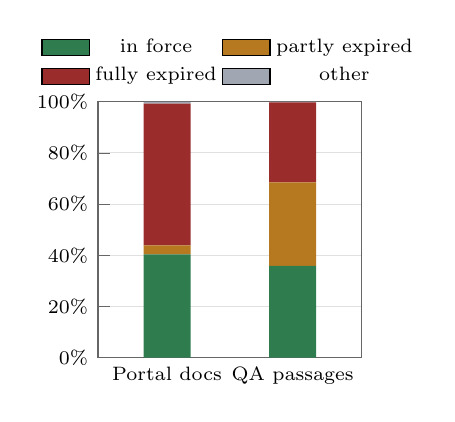
\begin{tikzpicture}
\begin{axis}[lexstyle, ybar stacked, scale only axis, width=3.35cm, height=3.25cm, bar width=17pt, ymin=0, ymax=100,
  symbolic x coords={pd,qa}, xtick=data, xticklabels={Portal docs,QA passages},
  yticklabel={\pgfmathprintnumber{\tick}\%}, enlarge x limits=0.55, area legend,
  legend style={at={(0.5,1.02)}, anchor=south, legend columns=2}, ymajorgrids]
\addplot[fill=cgreen, draw=none] coordinates {(pd,40.4) (qa,35.9)};
\addplot[fill=camber, draw=none] coordinates {(pd,3.5) (qa,32.6)};
\addplot[fill=cred, draw=none] coordinates {(pd,55.4) (qa,31.3)};
\addplot[fill=cgray, draw=none] coordinates {(pd,0.7) (qa,0.2)};
\legend{in force, partly expired, fully expired, other}
\end{axis}
\end{tikzpicture}
\end{minipage}
\caption{\textbf{The same question has different correct answers over time.} \emph{Left:} what LexGraph-VN answers when
the question is asked at each date (real system output). \emph{Right:} today 55\% of the 148,282 portal documents and
31\% of the 44,408 QA passages we link to them are no longer in force.}
\label{fig:teaser}
\end{figure}

\section{Introduction}
\label{sec:intro}
Vietnamese citizens ask legal questions every day: how many days of annual leave a worker gets, what the fine is for
running a red light, which papers a land transfer needs. The answers live in a large and fast-moving body of law. Laws
are guided by decrees, decrees by circulars; every year many of them are amended, replaced or repealed. A question
answering (QA) system that retrieves a repealed article gives a \emph{confidently wrong} answer, and standard retrieval
benchmarks, which pair each question with one fixed article, still count it as a hit.

Figure~\ref{fig:teaser} shows the problem on one question. The fine for a motorbike running a red light was
600.000--1.000.000 đồng under Decree 100/2019, became 800.000--1.000.000 đồng when Decree 123/2021 replaced the amount in
2022, and has been 4--6 million đồng since Decree 168/2024 replaced the whole article in 2025. All three answers are
correct, each at a different date. On the national legal portal, 55\% of documents are no longer in force, and 31\% of the
QA passages we can link to the portal come from documents that have fully expired.

We treat temporal legal QA as a \textbf{web mining} problem: the information that decides whether an article still
applies is spread over the \emph{content} of documents (``Sửa đổi điểm a khoản 3 Điều 6 như sau: \dots'') and the
\emph{link structure} between them (amends, replaces, repeals). LexGraph-VN mines both. Our contributions are:
\begin{itemize}
\item \textbf{A temporal legal knowledge graph, kept up to date.} We mine vbpl.vn into six relation types, a validity
interval for every document, \AmOps{} clause-level amendment operations and a learned \emph{version alignment} from old
articles to the articles that supersede them; a polite incremental crawler adds new documents and relations from the
portal (Section~\ref{sec:system}).
\item \textbf{A time-aware retrieval and answering pipeline.} Fine-tuned BGE-M3 and BGE-Reranker, successor injection
and a stale penalty retrieve the law in force at $t_q$, and a self-hosted Qwen3-4B writes a ``law changed'' notice only
from verified changes (Sections~\ref{sec:online}--\ref{sec:training}).
\item \textbf{A temporal evaluation.} The Stale@$k$ metric, metrics against the \emph{current} law, a time-travel test
that asks each question before and after its law changed, and an LLM-judged answer evaluation
(Section~\ref{sec:results}).
\end{itemize}
We ask three research questions. \textbf{RQ1}: how often are retrieved articles outdated, and how much do validity
signals fix it? \textbf{RQ2}: which relation types matter for finding the current law? \textbf{RQ3}: can a small
self-hosted LLM cite correctly and explain changes?



\textbf{Related work.} Retrieval-augmented generation~\citep{lewis2020rag} grounds an LLM on retrieved passages; dense
retrievers~\citep{karpukhin2020dpr,reimers2019sbert} and multilingual embedders such as BGE-M3~\citep{chen2024bgem3}
outperform BM25~\citep{robertson2009bm25} on Vietnamese legal retrieval, especially with semi-hard
negatives~\citep{le2025semihard} or synthetic data~\citep{son2024synthetic}. Legal IR benchmarks such as
COLIEE~\citep{rabelo2022coliee} treat statutes as fixed, while time-sensitive QA~\citep{chen2021timeqa,
zhang2021situatedqa,liska2022streamingqa} studies temporal context in open-domain text. We make time explicit for
statutes, where it is encoded in amending documents and in the portal's link structure.

% ===================================================================================================== 2
\section{System implementation}
\label{sec:system}

\begin{figure}[t]
\centering
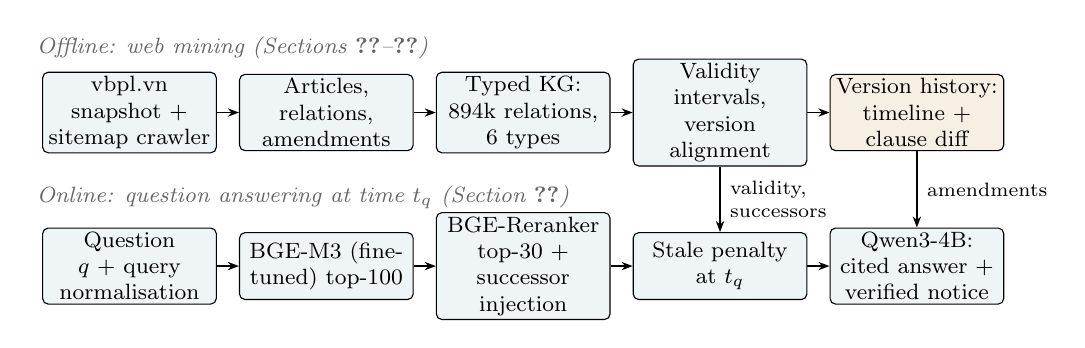
\begin{tikzpicture}[
  box/.style={draw, rounded corners=2pt, align=center, font=\footnotesize, text width=2.1cm,
              minimum height=0.85cm, inner sep=1.5pt, fill=cblue!7},
  arr/.style={-{Stealth[length=4pt]}, semithick},
  lane/.style={font=\footnotesize\itshape, anchor=west, text=black!60}]
\node[lane] at (-0.25, 0.82) {Offline: web mining (Sections~\ref{sec:data}--\ref{sec:temporal})};
\node[box] (crawl) at (1.05, 0)  {vbpl.vn snapshot + sitemap crawler};
\node[box] (ie)    at (3.55, 0)  {Articles, relations, amendments};
\node[box] (kg)    at (6.05, 0)  {Typed KG: 894k relations, 6 types};
\node[box] (time)  at (8.55, 0)  {Validity intervals, version alignment};
\node[box, fill=camber!12] (diff)  at (11.05, 0) {Version history: timeline + clause diff};
\node[lane] at (-0.25, -1.08) {Online: question answering at time $t_q$ (Section~\ref{sec:online})};
\node[box] (q)     at (1.05, -1.95)  {Question $q$ + query normalisation};
\node[box] (bi)    at (3.55, -1.95)  {BGE-M3 (fine-tuned) top-100};
\node[box] (ce)    at (6.05, -1.95)  {BGE-Reranker top-30 + successor injection};
\node[box] (rr)    at (8.55, -1.95)  {Stale penalty at $t_q$};
\node[box] (llm)   at (11.05, -1.95) {Qwen3-4B: cited answer + verified notice};
\draw[arr] (crawl) -- (ie); \draw[arr] (ie) -- (kg); \draw[arr] (kg) -- (time); \draw[arr] (time) -- (diff);
\draw[arr] (q) -- (bi); \draw[arr] (bi) -- (ce); \draw[arr] (ce) -- (rr); \draw[arr] (rr) -- (llm);
\draw[arr] (time) -- node[font=\scriptsize, right, align=left] {validity,\\successors} (rr);
\draw[arr] (diff) -- node[font=\scriptsize, right] {amendments} (llm);
\end{tikzpicture}
\caption{\textbf{LexGraph-VN pipeline.} \textbf{Offline}: the legal portal is mined into a knowledge graph with typed
relations, validity intervals, article versions and clause-level amendments, and kept up to date by a crawler.
\textbf{Online}: articles not in force at the question time $t_q$ move down, their newer versions move up, and Qwen3-4B
answers with citations.}
\label{fig:arch}
\end{figure}

LexGraph-VN must answer under the law in force at any date, cite clauses, explain changes, refuse without
evidence and stay up to date; it runs end to end on our own server (2$\times$H200, Figure~\ref{fig:arch}).

\subsection{Data}
\label{sec:data}
\textbf{Legal QA pairs.} 132,424 question--article pairs (119,007 questions, 68,663 passages). Questions are short
(\EdaQWords{} words on average), passages long (\EdaPWords{} words, 99th percentile \EdaPWordsNinetyNine), and
\EdaMultiGold{} of questions have two or more gold articles. Many questions are near-duplicates, so our split v2 groups
identical question texts: 95,231 / 11,891 / 11,885 questions for train / validation / test, with no question text in two
splits; \EdaUnseen{} of test gold passages are never seen in training.

\textbf{Legal portal.} The national legal database vbpl.vn publishes every normative document with metadata, full text
and relation lists. The redesigned portal serves relations only through an API that robots.txt disallows, so we start
from a public CC~BY~4.0 crawl (171,556 documents, 1,033,255 relation records), do all parsing and mining ourselves, and
add new documents with our own crawler. We keep 148,282 normative documents (\KgTypeDecision{} decisions,
\KgTypeResolution{} resolutions, \KgTypeCircular{} circulars, \KgTypeDecree{} decrees, \KgTypeLaw{} laws), dropping
translations, consolidated texts and administrative letters.

\begin{table}[t]
\centering
\caption{\textbf{Data at a glance.} The QA pairs supervise retrieval; the knowledge graph is mined from the portal.}
\label{tab:data}
\resizebox{\linewidth}{!}{%
\begin{tabular}{lr@{\hspace{2em}}lr}
\toprule
\multicolumn{2}{l}{\textbf{Legal QA pairs}} & \multicolumn{2}{l}{\textbf{Legal knowledge graph (web mining)}} \\
\midrule
Question--article pairs / questions & 132,424 / 119,007 & Documents / articles (\textit{Điều}) & 148,282 / 981,412 \\
Passages in the corpus & 68,663 & Typed edges (6 types) & 894,057 \\
Questions with $\geq$2 gold articles & \EdaMultiGold & Clause-level amendment operations & \AmOps \\
Split v2 train / val / test & 95,231 / 11,891 / 11,885 & QA passages linked to their article & 64.7\% \\
Test questions whose gold law has changed & \ResNTemporal & Passages with an aligned successor & \ResAlignAccepted \\
Words per question / passage & \EdaQWords{} / \EdaPWords & Documents added by our crawler & \LiveNewDocs \\
\bottomrule
\end{tabular}}
\end{table}

\subsection{Crawling the portal}
\label{sec:crawl}
\textbf{Politeness.} The crawler reads URLs and \texttt{lastmod} dates from the public sitemap (58,001 central documents),
fetches only \texttt{/van-ban/chi-tiet/} pages, and checks every URL against robots.txt with the longest-match rule of
RFC~9309~\citep{rfc9309} (Python's \texttt{robotparser} uses first match and would let \texttt{Allow: /} override
\texttt{Disallow: /api/}). It uses four workers with at least one second between requests, a generic research
User-Agent, retries with backoff and an on-disk cache. Of \CrawlFetched{} requests, \CrawlBlocked{} were blocked.

\textbf{Parsing.} Each page is server-rendered with a Next.js payload that contains the metadata object and the
full-text HTML. Against the public crawl on \ParserDocs{} documents present in both, the parser reproduces numbers,
titles, types and dates almost exactly (Figure~\ref{fig:crawl}a); status and issuing body differ more often because
the portal updates them over time.

\textbf{Relations from text.} Relation lists are not in the page, so we read them as a lawyer would: every document
number (including old formats such as \texttt{15/CP}), every citation by name and date (``Luật Tổ chức Chính phủ ngày 19
tháng 6 năm 2015'') and the Constitution are resolved to documents, duplicate numbers are disambiguated by the date
written next to them, and the sentence decides the type: ``Căn cứ'' lines give \emph{based on}; ``thay thế'' gives
\emph{replaces}; ``bãi bỏ'' or ``hết hiệu lực'' give \emph{repeals} (marked \emph{partial} when an article is
named); a sentence that performs ``Sửa đổi, bổ sung'' gives \emph{amends}; passive mentions (``đã được sửa đổi bởi'') are
only \emph{cites}. Against the portal's own lists on the same documents, any-type precision is 0.76 at recall 0.83
(Figure~\ref{fig:crawl}b).

\textbf{Incremental update.} New documents get a validity interval, articles, relations and amendment operations; an
older document that a new one replaces or repeals is closed at the new document's effective date; QA passages of
affected documents are aligned with the new articles; new articles are chunked and added to the corpus, and only their
embeddings are computed. One run on the November 2026 sitemap added \LiveNewDocs{} documents, \LiveNewArts{} articles,
\LiveNewEdges{} relations and \LiveNewOps{} amendment operations, and closed \LiveClosed{} older documents in two minutes.

\begin{figure}[t]
\centering
\begin{minipage}[t]{0.49\linewidth}\centering
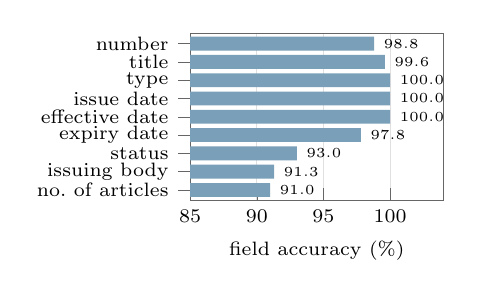
\begin{tikzpicture}
\begin{axis}[lexstyle, xbar, width=4.8cm, height=3.7cm, bar width=5pt, xmin=85, xmax=104,
  ytick=data, symbolic y coords/.expanded={\ParserSyms}, yticklabels/.expanded={\ParserLabels}, y dir=reverse,
  xmajorgrids, enlarge y limits=0.07, xlabel={field accuracy (\%)}, xtick={85,90,95,100},
  nodes near coords, nodes near coords style={font=\tiny, anchor=west}, point meta=rawx,
  every node near coord/.append style={/pgf/number format/.cd, fixed, precision=1, fixed zerofill}]
\addplot[fill=cblue!60, draw=none] coordinates {\ParserCoords};
\end{axis}
\end{tikzpicture}\\
{\footnotesize (a) Page parser vs.\ the public crawl}
\end{minipage}\hfill
\begin{minipage}[t]{0.49\linewidth}\centering
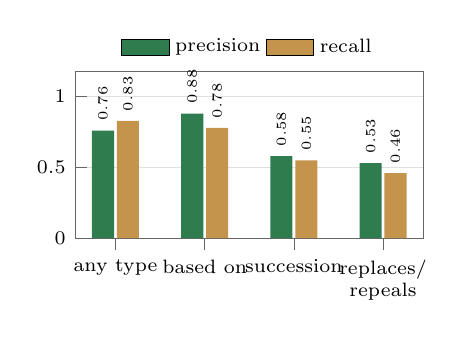
\begin{tikzpicture}
\begin{axis}[lexstyle, ybar=1pt, width=6.0cm, height=3.7cm, bar width=8pt, ymin=0, ymax=1.18, ytick={0,0.5,1},
  symbolic x coords/.expanded={\RelSyms}, xticklabels={any type, based on, succession, {replaces/\\repeals}}, xtick=data,
  xticklabel style={align=center, font=\scriptsize},
  ymajorgrids, enlarge x limits=0.15, legend style={at={(0.5,1.02)}, anchor=south, legend columns=2}, area legend,
  nodes near coords, nodes near coords style={font=\tiny, rotate=90, anchor=west}, point meta=rawy,
  every node near coord/.append style={/pgf/number format/.cd, fixed, precision=2, fixed zerofill}]
\addplot[fill=cgreen, draw=none] coordinates {\RelP};
\addplot[fill=camber!80, draw=none] coordinates {\RelR};
\legend{precision, recall}
\end{axis}
\end{tikzpicture}\\
{\footnotesize (b) Relations from text vs.\ the portal's lists}
\end{minipage}
\caption{\textbf{Crawler evaluation} on \ParserDocs{} documents present in both the public crawl and our crawl.
(a) Accuracy of each metadata field and of the article split. (b) Relations extracted from the text against the
portal's own relation lists, by target document; succession: amends, replaces, repeals.}
\label{fig:crawl}
\end{figure}

\subsection{Knowledge graph}
\label{sec:kg}
\textbf{Typed relations.} The portal lists relations from each document's own page, so the direction of a label depends
on the page (``Văn bản bị thay thế'' vs.\ ``Văn bản thay thế''). We map 19 labels to six typed edges
\emph{actor$\to$target} (based on, cites, guides, amends, replaces, repeals) and verify each direction with issue
dates: the actor is newer than the target in 97--100\% of edges per label. A partial repeal (6,557 edges) is a
\emph{repeals} edge marked \emph{partial}: it ends some articles but not the document. Labels too rare to matter are
left out (suspension: 188 edges, interpretation: 85; consolidation links point to consolidated texts, which we exclude).
Figure~\ref{fig:kg}a shows the distribution; succession edges (amends, replaces, repeals) make up 13.7\% of all edges
but decide validity.

\textbf{The links decide validity.} An article never says in its own text that it has been superseded; only other
documents do, through their links. The first replaces or (full) repeals edge that points at a document closes its validity
interval, and the candidate successors of an article are found by following amends, replaces and repeals edges (up to
two hops). The typed link structure is therefore not an add-on to retrieval but the source of the temporal signal:
Section~\ref{sec:ablation} shows that dropping either family of succession edges lowers retrieval under the current law.

\textbf{Articles and references.} HTML is split into 981,412 articles from \KgDocsWithArticles{} documents. Rules extract
document and article references; against the portal's (incomplete) lists, document references reach precision \KgXrefP{}
and recall \KgXrefR{}, and \KgXrefNew{} extracted references are not in the portal's lists at all. \KgArtXrefRes\% of
\KgArtXref{} article-level references resolve to an article in the graph. QA passages are linked to their source article
by heading and token containment (64.7\% linked).

\textbf{Link analysis.} Louvain~\citep{blondel2008louvain} on the citation graph (\KgLouvainNodes{} documents) finds
\KgLouvainComm{} communities with modularity \KgLouvainMod{}; the largest match legal domains (state budget,
labour and wages, tax and fees, organisation and civil service, import--export, land and prices). HITS
authorities~\citep{kleinberg1999hits} are the framework laws on local government, on legal normative documents and on
the state budget.

\textbf{Clause-level amendments.} Amending documents state their changes as operations: ``a) Sửa đổi điểm a khoản 3
Điều 6 như sau: \dots'', ``Bãi bỏ điểm đ khoản 4 Điều 6'', ``Thay cụm từ `600.000 đồng đến 1.000.000 đồng' bằng cụm từ
`800.000 đồng đến 1.000.000 đồng' tại khoản 4 Điều 6, khoản 5 Điều 47''. We parse \AmOps{} operations from \AmDocs{}
documents (Figure~\ref{fig:kg}b) into (operation, article, clause, point, new text); a phrase replacement with several
targets becomes one operation per target. The target document is resolved for \AmResolved\% of operations and the
target article found for \AmArtFound\%. These operations are applied at question time (Section~\ref{sec:online}) and
drive the version history of the demo.

\begin{figure}[t]
\centering
\begin{minipage}[t]{0.49\linewidth}\centering
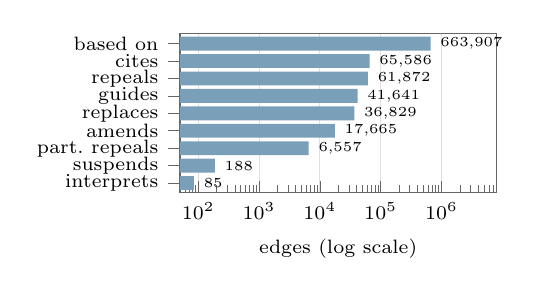
\begin{tikzpicture}
\begin{axis}[lexstyle, xbar, width=5.6cm, height=3.6cm, bar width=5pt, xmode=log, xmin=50, xmax=8e6,
  ytick=data, symbolic y coords/.expanded={\KgEdgeSyms}, yticklabels/.expanded={\KgEdgeLabels}, y dir=reverse,
  xmajorgrids, enlarge y limits=0.07, xlabel={edges (log scale)},
  nodes near coords={\pgfmathprintnumber[fixed, precision=0, 1000 sep={\text{,}}]{\pgfplotspointmeta}},
  nodes near coords style={font=\tiny, anchor=west}, point meta=rawx]
\addplot[fill=cblue!60, draw=none] coordinates {\KgEdgeCoords};
\end{axis}
\end{tikzpicture}\\
{\footnotesize (a) Typed relations (894,057 edges)}
\end{minipage}\hfill
\begin{minipage}[t]{0.49\linewidth}\centering
\begin{tikzpicture}
\begin{axis}[lexstyle, xbar, width=5.2cm, height=3.6cm, bar width=6pt, xmin=0,
  symbolic y coords={{Sửa đổi, bổ sung},{Sửa đổi},{Bổ sung},{Bãi bỏ},{Thay thế},{Thay cụm từ}}, ytick=data, y dir=reverse,
  xmajorgrids, enlarge y limits=0.1, xlabel={operations}, scaled x ticks=false, xtick={0,10000,20000},
  xticklabel style={/pgf/number format/1000 sep={\text{,}}}, xmax=22500,
  nodes near coords={\pgfmathprintnumber[fixed, precision=0, 1000 sep={\text{,}}]{\pgfplotspointmeta}},
  nodes near coords style={font=\tiny, anchor=west}, point meta=rawx]
\addplot[fill=camber!80, draw=none] coordinates {\AmOpCoords};
\end{axis}
\end{tikzpicture}\\
{\footnotesize (b) Clause-level amendment operations (\AmOps)}
\end{minipage}
\caption{\textbf{What the portal tells us.} (a) The six edge types of the knowledge graph; succession edges (amends,
replaces, repeals) decide validity. (b) Operations parsed from amending documents.}
\label{fig:kg}
\end{figure}

\subsection{Temporal layer}
\label{sec:temporal}
\textbf{Validity.} Each document $D$ gets an interval $[v_{\mathrm{from}}(D), v_{\mathrm{to}}(D))$ from its effective and
expiry dates, its status, and the effective date of the first document that replaces or repeals it. An article $a$ of
$D$ is \emph{stale} at time $t$ if
\[
t \notin [v_{\mathrm{from}}(D), v_{\mathrm{to}}(D)) \quad \text{or} \quad \exists\, a' \in \mathrm{succ}(a):\;
v_{\mathrm{from}}(\mathrm{doc}(a')) \leq t ,
\]
where $\mathrm{succ}(a)$ are the articles aligned with $a$ in documents that amend, replace or repeal $D$.

\textbf{Version alignment.} For each QA passage of a document with successors, the candidates are the three most
similar articles (bi-encoder cosine) in every amending, replacing or repealing document within two hops (31,574
passages, \ResAlignArtPairs{} article pairs). Which of them really supersedes the old article? We label
\ResAlignJudged{} stratified pairs with gpt-oss-120b~\citep{gptoss2025} as a judge~\citep{zheng2023judge}
(\AlPosRate{} positive; split by old document \AlSplits), train a gradient-boosting classifier~\citep{friedman2001gbm}
on pair features (Figure~\ref{fig:align}b), and match old and new articles one to one with the Hungarian
algorithm~\citep{kuhn1955hungarian} within each (old document, new document) pair, keeping a match when its
probability is at least \ResAlignThr. On judged test pairs, accepted links have precision \ResAlignPrec{} (classifier
alone: \AlClsP{} at recall \AlClsR); \ResAlignArtAccepted{} article pairs are matched and \ResAlignAccepted{} of 31,574
passages get a successor (Figure~\ref{fig:align}a). Similarity and lexical overlap carry most of the signal; the
relation type and clause-level operations help for the remaining cases.

\begin{figure}[t]
\centering
\begin{minipage}[t]{0.49\linewidth}\centering
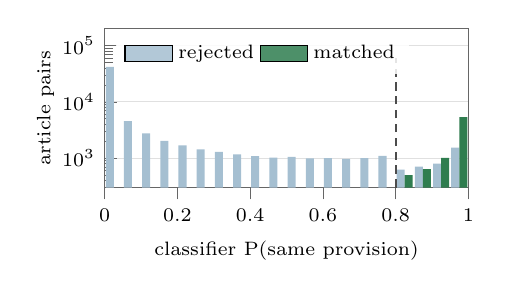
\begin{tikzpicture}
\begin{axis}[lexstyle, ybar=0pt, width=6.2cm, height=3.6cm, bar width=2.9pt, xmin=0, xmax=1.0, ymode=log, ymin=300,
  ymax=200000, xlabel={classifier P(same provision)}, ylabel={article pairs}, ymajorgrids,
  ylabel shift=-4pt, legend style={at={(0.03,0.97)}, anchor=north west, fill=white, fill opacity=0.85, text opacity=1,
  legend columns=2}, area legend, log origin=infty, unbounded coords=discard]
\addplot[fill=cblue!40, draw=none] coordinates {\ResAlignHistRej};
\addplot[fill=cgreen, draw=none] coordinates {\ResAlignHistAcc};
\draw[densely dashed, thick, black!70] (axis cs:\ResAlignThr,300) -- (axis cs:\ResAlignThr,60000);
\legend{rejected, matched}
\end{axis}
\end{tikzpicture}\\
{\footnotesize (a) Candidate pairs and one-to-one matches}
\end{minipage}\hfill
\begin{minipage}[t]{0.49\linewidth}\centering
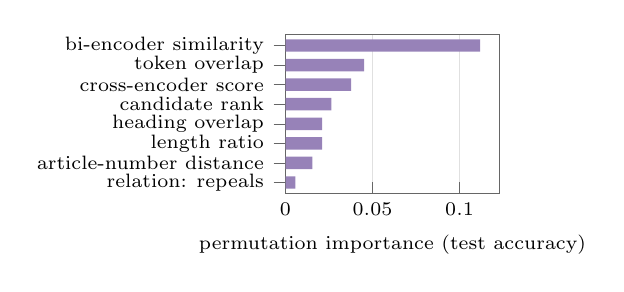
\begin{tikzpicture}
\begin{axis}[lexstyle, xbar, width=4.3cm, height=3.6cm, bar width=4.5pt, xmin=0,
  ytick=data, symbolic y coords/.expanded={\AlFeatSyms}, yticklabels/.expanded={\AlFeatLabels}, y dir=reverse,
  xmajorgrids, enlarge y limits=0.08, xlabel={permutation importance (test accuracy)},
  xticklabel style={/pgf/number format/fixed, /pgf/number format/precision=2}, scaled x ticks=false]
\addplot[fill=cpurple!70, draw=none] coordinates {\AlFeatCoords};
\end{axis}
\end{tikzpicture}\\
{\footnotesize (b) Most useful pair features}
\end{minipage}
\caption{\textbf{Version alignment.} (a) Classifier probability of the \ResAlignArtPairs{} candidate (old, new) article
pairs; one-to-one matching keeps \ResAlignArtAccepted{} pairs above the threshold (dashed). (b) Drop in test accuracy
when a feature is shuffled.}
\label{fig:align}
\end{figure}

\subsection{Online question answering}
\label{sec:online}
\textbf{Query normalisation.} Citizens and the law use different words: ``vượt đèn đỏ'' vs.\ ``không chấp hành hiệu lệnh
của đèn tín hiệu giao thông''. A small glossary appends the legal phrase to the question before retrieval.

\textbf{Retrieval and re-ranking.} The fine-tuned BGE-M3 bi-encoder returns the top-100 chunks of the extended corpus (QA
passages plus 116,553 chunks of successor articles). The fine-tuned BGE-Reranker scores the top-30 plus the successors
of stale candidates (\emph{successor injection}), so the current version can be found even when only the old one was
retrieved. The final score subtracts a stale penalty:
\[
s(q, d, t_q) = s_{\mathrm{CE}}(q, d) - \gamma \, \mathbf{1}\left[d \text{ is stale at } t_q\right],
\]
with $\gamma$ tuned on validation (Section~\ref{sec:ablation}).

\textbf{Context.} For each of the top five articles in force, Qwen3-4B receives the clause most relevant to the
question (cross-encoder over clause chunks, with a bonus for exact legal phrases), its validity, and the amendment
operations in force at $t_q$: phrase replacements are applied to the text inside their target clause (so a question
asked in 2023 sees ``800.000 đồng đến 1.000.000 đồng''), and other operations on the clauses shown are appended.

\textbf{Verified change notices.} A ``Thay đổi pháp luật'' (law changed) section is only allowed from a \emph{verified change fact}.
For the most relevant stale article, we compare the clause the question is about (old version just before the successor
took effect, phrase replacements applied) with the most relevant clause of its successor. The fact is kept if the fine
amounts differ or the token Jaccard similarity is below 0.85, \emph{and} Qwen3-4B confirms, in a one-word answer, that
the answer to the question differs. The fact is given to the model in a separate block; after generation, a notice
without a fact is removed and a missing one is added. The model must cite document, article and clause as $[k]$ and
answer ``Không tìm thấy đủ căn cứ pháp lý'' when the sources do not cover the question. Qwen3-4B~\citep{qwen3} runs in
non-thinking mode on vLLM~\citep{kwon2023vllm}.

\textbf{Demo.} A Streamlit app answers at any date, compares three dates side by side, marks validity and newly
crawled documents, and shows each article's version history with word-level clause diffs.

% ===================================================================================================== 3
\section{Training}
\label{sec:training}
\textbf{Negative mining.} Following~\citet{le2025semihard}, negatives are \emph{semi-hard}: from the top-100 of a
retriever, we skip the first three ranks and any candidate scoring within 0.05 of the positive (likely unlabelled positives),
and keep the next ones. The bi-encoder gets 3 negatives per pair mined with the zero-shot BGE-M3; the cross-encoder gets
7 negatives per question mined with the \emph{fine-tuned} BGE-M3, so it learns to separate what the final retriever
actually confuses.

\textbf{Objectives.} The bi-encoder is trained with the multiple-negatives ranking loss~\citep{henderson2017mnrl}, which
treats the other positives in the batch (gathered across both GPUs) and the mined negatives as negatives:
\[
\mathcal{L}_{\mathrm{bi}} = -\frac{1}{B}\sum_{i=1}^{B} \log
\frac{\exp\left(\lambda \cos(q_i, p_i)\right)}{\sum_{j=1}^{B} \exp\left(\lambda \cos(q_i, p_j)\right) + \sum_{n \in N_i} \exp\left(\lambda \cos(q_i, n)\right)},
\qquad \lambda = 20 .
\]
The cross-encoder is trained with binary cross-entropy on (question, passage) pairs, with the positive class weighted by
7 to balance one positive against seven negatives.

\begin{table}[t]
\centering
\caption{\textbf{Fine-tuning setup.} Both models: one epoch, bf16, DDP on 2$\times$H200, linear schedule with 10\% warm-up,
seed 42, best checkpoint on validation.}
\label{tab:train}
\small
\begin{tabular}{lll}
\toprule
& \textbf{Bi-encoder} & \textbf{Cross-encoder} \\
\midrule
Initialisation & BAAI/bge-m3 (568M) & BAAI/bge-reranker-v2-m3 (568M) \\
Loss & multiple-negatives ranking, $\lambda = 20$ & binary cross-entropy, positive weight 7 \\
Training data & 105,899 pairs + 3 negatives & \ResCePairs{} pairs (1 positive + 7 negatives) \\
Negatives mined with & zero-shot BGE-M3, top-100 & fine-tuned BGE-M3, top-100 \\
Batch / learning rate & 128 questions (64 per GPU) / $10^{-5}$ & 128 pairs (64 per GPU) / $10^{-5}$ \\
Max length & 512 tokens, gradient checkpointing & 512 tokens \\
Validation & MRR@10, 2,000 questions, every 200 steps & MRR@10 over top-30, 1,000 questions \\
Training time & $\approx$25 min & $\approx$30 min \\
\bottomrule
\end{tabular}
\end{table}

\begin{wrapfigure}{r}{0.42\linewidth}
\vspace{-4mm}
\centering
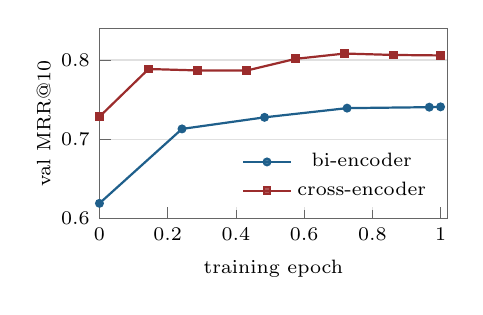
\begin{tikzpicture}
\begin{axis}[lexstyle, width=6.0cm, height=4.0cm, xmin=0, xmax=1.02, ymin=0.6, ymax=0.84, xlabel={training epoch},
  ylabel={val MRR@10}, ymajorgrids, legend style={at={(0.98,0.04)}, anchor=south east, fill=white, fill opacity=0.8,
  text opacity=1}, ylabel shift=-3pt]
\addplot[cblue, thick, mark=*, mark size=1.2pt] coordinates {\ResBiCurve};
\addplot[cred, thick, mark=square*, mark size=1.2pt] coordinates {\ResCeCurve};
\legend{bi-encoder, cross-encoder}
\end{axis}
\end{tikzpicture}
\vspace{-2mm}
\caption{Validation MRR@10 during fine-tuning (epoch 0: zero-shot).}
\label{fig:curves}
\vspace{-4mm}
\end{wrapfigure}
\textbf{Engineering.} Training uses Sentence-Transformers with DDP (the unused XLM-R pooler requires
unused-parameter detection) and non-reentrant gradient checkpointing to fit 64 questions $\times$ 5 texts $\times$ 512
tokens per GPU; Table~\ref{tab:train} lists the setup. Figure~\ref{fig:curves} shows that most of the gain comes in the first
quarter of the epoch: the bi-encoder rises from 0.619 to 0.741 validation MRR@10 (Recall@100 from 0.930 to 0.980), and
the fine-tuned cross-encoder reaches 0.808 over the bi-encoder's top-30 (zero-shot: 0.729).

% ===================================================================================================== 4
\section{Main results}
\label{sec:results}
\paragraph{Setup: we grade against today's law.}
All results use the 11,885 test questions of split v2 at $t = $ 23/11/2026. Besides MRR@10 and Recall@$k$ against the
original gold, we report metrics against the \emph{current} gold (a superseded gold passage is replaced by its successor;
subscript ``cur'') and the share of outdated results
\[
\mathrm{Stale@}k = \frac{1}{\lvert Q \rvert} \sum_{q \in Q} \frac{1}{k} \sum_{d \in \mathrm{top}\text{-}k(q)}
\mathbf{1}\left[d \text{ is stale at } t\right].
\]
``T-'' metrics use the \ResNTemporal{} test questions whose gold article was superseded.

\begin{table}[t]
\centering
\caption{\textbf{Retrieval} (11,885 test questions). \emph{Left:} retrieval only on the QA corpus (68,663 passages).
\emph{Right:} the extended corpus used by the system (185,216 chunks, also holding the successor articles).}
\label{tab:retrieval}
\small
\begin{minipage}[t]{0.485\linewidth}\centering
\resizebox{\linewidth}{!}{%
\begin{tabular}{lccc}
\toprule
Method & MRR@10 & R@10 & R@100 \\
\midrule
\BaseRows
\bottomrule
\end{tabular}}
\end{minipage}\hfill
\begin{minipage}[t]{0.485\linewidth}\centering
\resizebox{\linewidth}{!}{%
\begin{tabular}{lccc}
\toprule
Method & MRR@10 & R@10 & R@100 \\
\midrule
BGE-M3 (zero-shot) & \ResZsMrr & \ResZsRten & 0.900 \\
\quad + BGE-Reranker & \ResZsCeMrr & \ResZsCeRten & -- \\
BGE-M3 (fine-tuned) & \ResFtMrr & \ResFtRten & 0.972 \\
\quad \textbf{+ BGE-Reranker (FT)} & \textbf{\ResFtCeMrr} & \textbf{\ResFtCeRten} & -- \\
\bottomrule
\end{tabular}}
\end{minipage}
\end{table}

\paragraph{Fine-tuning pays off.}
Dense retrieval clearly beats lexical matching: on the QA corpus, zero-shot BGE-M3 reaches 0.608 MRR@10 against 0.491
for the best BM25, and fine-tuning lifts it to 0.725 (Table~\ref{tab:retrieval}). The system searches the larger
extended corpus, which also holds the successor articles, so absolute numbers are lower there. Re-ranking matters as
much as retrieval: the zero-shot reranker adds 0.085 MRR@10, and fine-tuning both models adds another 0.080, to
\textbf{\ResFtCeMrr} MRR@10.



\paragraph{RQ1: validity signals halve outdated results.}
Without them, \ResStaleNoTimePct{} of the top-10 results are no longer in force; with the stale penalty and successor
injection, \ResStaleTimePct{} (Table~\ref{tab:abl}). MRR@10 under the current law on changed questions rises from
\ResTmrrNoTime{} to \ResTmrrTime. MRR@10 against the \emph{original} gold drops from \ResFtCeMrr{} to \ResTimeMrr{}, as
intended: the system now prefers the newer article the static benchmark does not know.

\begin{table}[t]
\centering
\caption{\textbf{Validity signals and ablations} (fine-tuned models, test). ``cur'': gold replaced by its successor if
superseded; T: the \ResNTemporal{} changed questions; Stale@10: share of the top 10 not in force on 23/11/2026; \ResWeights{}
chosen on validation.}
\label{tab:abl}
\setlength{\tabcolsep}{5pt}
\resizebox{\linewidth}{!}{%
\begin{tabular}{lccccc}
\toprule
System & MRR@10 & MRR@10$\cur$ & Stale@10 $\downarrow$ & T-MRR@10$\cur$ & T-Hit@10$\cur$ \\
\midrule
\ResAblRows
\bottomrule
\end{tabular}}
\end{table}

\subsection{Ablation studies}
\label{sec:ablation}
\paragraph{A moderate penalty is enough.}
Stale@10 keeps falling as $\gamma$ grows (Figure~\ref{fig:results}a), but beyond $\gamma = 2$ the penalty also hides old
articles that are still the best evidence for an unchanged clause, and MRR@10$\cur$ drops; we use $\gamma = 2$. The
penalty alone is not enough: without \emph{successor injection}, T-Hit@10$\cur$ falls from \ResThitTime{} to 0.721,
because the bi-encoder often retrieves only the old version and the new article never reaches the re-ranker.

\paragraph{RQ2: the links decide what is current.}
Keeping only amends edges, or only replaces / repeals edges, lowers T-MRR@10$\cur$ to \ResTmrrAmends{} and
\ResTmrrRepl{}: the two families cover different changes and both are needed. The \emph{link structure} of the portal,
not the text of the articles, tells the system which article is current. (The lower Stale@10 of these variants is not
a gain: fewer successors means fewer articles marked as stale.)

\begin{figure}[t]
\centering
\pgfplotsset{panel/.style={lexstyle, scale only axis, width=3.55cm, height=2.4cm}}
\begin{minipage}[t]{0.325\linewidth}\centering
\begin{tikzpicture}
\begin{axis}[panel, width=2.55cm, xmode=log, log basis x=2, xmin=0.4, xmax=10, xtick={0.5,1,2,4,8}, xticklabels={0.5,1,2,4,8},
  xlabel={stale penalty $\gamma$}, ylabel={val MRR@10$\cur$}, ymin=0.645, ymax=0.71, ymajorgrids, ytick={0.65,0.67,0.69},
  axis y line*=left, ylabel shift=-3pt, yticklabel style={/pgf/number format/fixed, /pgf/number format/precision=2}]
\addplot[cgreen, thick, mark=*, mark size=1.3pt] coordinates {\ResGammaMrr}; \label{pl:gm}
\end{axis}
\begin{axis}[panel, width=2.55cm, xmode=log, log basis x=2, xmin=0.4, xmax=10, axis y line*=right, axis x line=none,
  ytick pos=right, yticklabel pos=right, ylabel near ticks, ylabel={Stale@10}, ymin=0, ymax=0.3, ytick={0,0.1,0.2,0.3},
  legend style={at={(0.5,1.02)}, anchor=south, legend columns=2}]
\addlegendimage{/pgfplots/refstyle=pl:gm}\addlegendentry{MRR@10$\cur$}
\addplot[camber, thick, dashed, mark=triangle*, mark size=1.4pt] coordinates {\ResGammaStale};
\addlegendentry{Stale@10}
\end{axis}
\end{tikzpicture}\\[-0.5mm]
{\footnotesize (a) Stale penalty $\gamma$ (validation)}
\end{minipage}\hfill
\begin{minipage}[t]{0.325\linewidth}\centering
\begin{tikzpicture}
\begin{axis}[panel, ybar, bar width=7pt, ymin=0, ymax=0.9,
  symbolic x coords={st,tt,tm}, xtick=data,
  xticklabels={{Stale@10$\downarrow$},{T-MRR$\cur$},{T-Hit@10$\cur$}},
  ymajorgrids, enlarge x limits=0.25, legend style={at={(0.5,1.02)}, anchor=south, legend columns=2}, area legend,
  nodes near coords, nodes near coords style={font=\tiny}, point meta=explicit symbolic]
\addplot[fill=cgray, draw=none, nodes near coords style={font=\tiny, anchor=south east, xshift=2pt}] coordinates {(st,\ResStaleNoTime) [\ResStaleNoTime] (tt,\ResTmrrNoTime) [\ResTmrrNoTime] (tm,\ResThitNoTime) [\ResThitNoTime]};
\addplot[fill=cgreen, draw=none, nodes near coords style={font=\tiny, anchor=south west, xshift=-2pt}] coordinates {(st,\ResStaleTime) [\ResStaleTime] (tt,\ResTmrrTime) [\ResTmrrTime] (tm,\ResThitTime) [\ResThitTime]};
\legend{no time signals, with time signals}
\end{axis}
\end{tikzpicture}\\[-0.5mm]
{\footnotesize (b) Changed questions (test)}
\end{minipage}\hfill
\begin{minipage}[t]{0.325\linewidth}\centering
\begin{tikzpicture}
\begin{axis}[panel, ybar, bar width=5pt, ymin=0, ymax=1.05,
  symbolic x coords={before,after,both}, xtick=data, xticklabels={before,after,both},
  ylabel={Hit@10}, ymajorgrids, enlarge x limits=0.22, ylabel shift=-3pt,
  legend style={at={(0.5,1.02)}, anchor=south, legend columns=3}, area legend]
\addplot[fill=cgray, draw=none] coordinates {\ResTtSt};
\addplot[fill=cblue!45, draw=none] coordinates {\ResTtNt};
\addplot[fill=cgreen, draw=none] coordinates {\ResTtLg};
\legend{static, no time, ours}
\end{axis}
\end{tikzpicture}\\[-0.5mm]
{\footnotesize (c) Time-travel (\ResNTt{} questions)}
\end{minipage}
\caption{\textbf{Validity signals fix outdated answers.} (a) Beyond $\gamma{=}2$ the penalty also hides useful context.
(b) The \ResNTemporal{} test questions whose gold article was superseded. (c) Hit@10 when each question is asked the day
before its successor took effect (gold: the old article) and on 23/11/2026 (gold: the new one).}
\label{fig:results}
\end{figure}

\begin{figure}[t]
\centering
\begin{minipage}[t]{0.49\linewidth}\centering
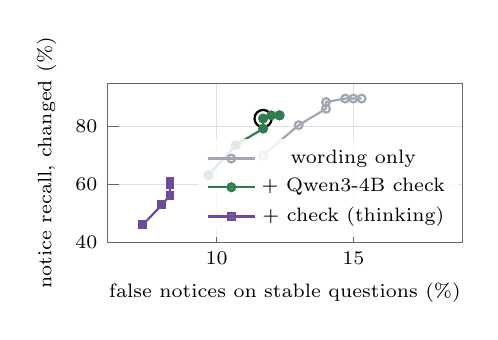
\begin{tikzpicture}
\begin{axis}[lexstyle, width=6.1cm, height=3.6cm, xmin=6, xmax=19, ymin=40, ymax=95, xlabel={false notices on stable questions (\%)},
  ylabel={notice recall, changed (\%)}, ymajorgrids, xmajorgrids, legend style={at={(0.99,0.03)}, anchor=south east,
  fill=white, fill opacity=0.85, text opacity=1}]
\addplot[cgray, thick, mark=o, mark size=1.4pt] coordinates {\NoticeNone};
\addplot[cgreen, thick, mark=*, mark size=1.4pt] coordinates {\NoticeFast};
\addplot[cpurple, thick, mark=square*, mark size=1.2pt] coordinates {\NoticeThink};
\node[draw=black, circle, inner sep=2.2pt, thick] at (axis cs:11.7,82.8) {};
\legend{wording only, + Qwen3-4B check, + check (thinking)}
\end{axis}
\end{tikzpicture}\\
{\footnotesize (a) Change notices: false alarms vs.\ recall (validation)}
\end{minipage}\hfill
\begin{minipage}[t]{0.49\linewidth}\centering
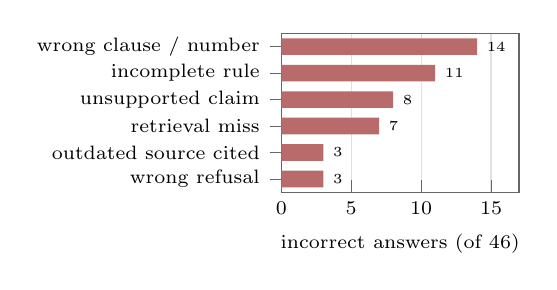
\begin{tikzpicture}
\begin{axis}[lexstyle, xbar, width=4.6cm, height=3.6cm, bar width=6pt, xmin=0, xmax=17,
  ytick=data, symbolic y coords/.expanded={\FmSyms}, yticklabels/.expanded={\FmLabels}, y dir=reverse,
  xmajorgrids, enlarge y limits=0.1, xlabel={incorrect answers (of \FmWrong)},
  nodes near coords, nodes near coords style={font=\tiny, anchor=west}, point meta=rawx]
\addplot[fill=cred!70, draw=none] coordinates {\FmCoords};
\end{axis}
\end{tikzpicture}\\
{\footnotesize (b) Failure modes of time-aware answers (test)}
\end{minipage}
\caption{\textbf{Where the system still fails.} (a) Notice rules on validation; points: Jaccard threshold 0.6--1.0,
circle: chosen. (b) Causes of the \FmWrong{} incorrect answers; the first three had the gold article in context.}
\label{fig:notice}
\end{figure}

\paragraph{Right before and after the change.}
A static system can only be right once. We ask each of \ResNTt{} changed questions twice: the day before its successor
took effect (gold: the old article) and on 23/11/2026 (gold: the new one; Figure~\ref{fig:results}c). Static RAG is
right before the change (0.917) but almost never after (0.060). The extended corpus without validity signals finds the
new article more often but keeps mixing in old ones; LexGraph-VN is right at \emph{both} dates for \ResTtBothPct{} of
questions (static RAG: \ResTtStaticBothPct).

\begin{figure}[t]
\centering
\pgfplotsset{ans/.style={lexstyle, ybar=0.6pt, width=6.4cm, height=3.4cm, bar width=6.5pt, ymin=0, ymax=1.42,
  ytick={0,0.25,0.5,0.75,1}, ymajorgrids, enlarge x limits=0.14, xtick=data,
  xticklabel style={align=center, font=\scriptsize}, nodes near coords, point meta=rawy,
  nodes near coords style={font=\tiny, rotate=90, anchor=west, /pgf/number format/.cd, fixed, precision=2, fixed zerofill},
  legend style={at={(0.5,1.03)}, anchor=south, legend columns=3}, area legend}}
\begin{minipage}[t]{0.49\linewidth}\centering
\begin{tikzpicture}
\begin{axis}[ans, symbolic x coords={goall,gochg,qwall,qwchg},
  xticklabels={{all\\\textit{gpt-oss}}, {changed\\\textit{gpt-oss}}, {all\\\textit{Qwen3-32B}}, {changed\\\textit{Qwen3-32B}}}]
\addplot[fill=cgray, draw=none] coordinates {\AnsANone};
\addplot[fill=cblue!45, draw=none] coordinates {\AnsAPlain};
\addplot[fill=cgreen, draw=none] coordinates {\AnsAOurs};
\legend{no retrieval, plain RAG, time-aware (ours)}
\end{axis}
\end{tikzpicture}\\
{\footnotesize (a) Judged correct, by judge}
\end{minipage}\hfill
\begin{minipage}[t]{0.49\linewidth}\centering
\begin{tikzpicture}
\begin{axis}[ans, symbolic x coords={cite,faith,faithq,refuse},
  xticklabels={{cites current\\gold article}, {faithful\\\textit{gpt-oss}}, {faithful\\\textit{Qwen3-32B}}, {refuses out\\of scope}}]
\addplot[fill=cgray, draw=none] coordinates {\AnsBNone};
\addplot[fill=cblue!45, draw=none] coordinates {\AnsBPlain};
\addplot[fill=cgreen, draw=none] coordinates {\AnsBOurs};
\legend{no retrieval, plain RAG, time-aware (ours)}
\end{axis}
\end{tikzpicture}\\
{\footnotesize (b) Citations, faithfulness and refusals}
\end{minipage}
\caption{\textbf{Qwen3-4B answers} on \ResNAns{} questions (100 stable, 50 changed, 20 out of scope), graded by two LLM
judges. Time-aware RAG is the most correct under both judges, especially on changed questions. Without retrieval the
model cites nothing.}
\label{fig:answers}
\end{figure}

\paragraph{RQ3: better answers, confirmed by two judges.}
Qwen3-4B answers 100 stable, 50 changed and 20 out-of-scope questions without retrieval, with plain RAG and with
LexGraph-VN, graded by gpt-oss-120b. Time-aware RAG is the most correct (\ResAnsCorrect{} vs.\ \ResAnsPlainCorrect{}
plain, \ResAnsNoneCorrectPct{} without retrieval) and cites current articles more often (Figure~\ref{fig:answers}). A
second judge, Qwen3-32B, ranks the settings the same way; the judges agree on \JTwoAgreeCorrect{} of correctness labels
($\kappa = \JTwoKappaCorrect$) and \JTwoAgreeFaithful{} of faithfulness labels ($\kappa = \JTwoKappaFaithful$).


\paragraph{Fewer false alarms, at a price.}
Notices reach \ResAnsNoticeRecallPct{} of really changed answers with \ResAnsFalseAlarmPct{} false notices on stable
questions. On validation (Figure~\ref{fig:notice}a), a looser Jaccard threshold buys recall with false alarms; a one-word
Qwen3-4B check removes a sixth of them at a small recall cost (we use Jaccard $<0.85$ with this check). Recall is capped
near 0.90: for 10\% of changed questions the old article is never retrieved.

\paragraph{Errors come from reading, not retrieval.}
Of the \FmWrong{} incorrect answers (Figure~\ref{fig:notice}b), only \FmRetrieval{} lack a current gold article in the
context and \FmOutdated{} cite an outdated source. \FmMisread{} have the right article yet pick another clause or amount
(\FmClause), state the rule incompletely (\FmIncomplete) or add unsupported content (\FmUnsupported); \FmRefusal{}
refuse wrongly. All \FmMissedNoFact{} missed notices lacked the old article; the \FmFalse{} false notices come from
stale articles other than the gold one.

% ===================================================================================================== 5
\section{Conclusion}
\label{sec:conclusion}
LexGraph-VN shows that temporal validity is a first-class problem for legal QA, and that the content and link
structure of a legal portal can solve much of it: validity signals almost halve outdated results, raise retrieval under
the current law on changed questions by 0.11 MRR@10, and make the system right before and after a change for
\ResTtBothPct{} of questions (static RAG: \ResTtStaticBothPct).

\textbf{Limitations and future work.} 35\% of QA passages are not linked to the portal; alignment favours precision
(recall 0.33); notices still have 13\% false alarms; answers are judged by LLMs on 170 questions. Next steps are old
versions as hard negatives, higher alignment recall, and claim-level citation checks with NLI.

\bibliography{references}
\bibliographystyle{iclr2027_conference}

\end{document}
